\subsection{IXMUX} \label{subsec:IXMUX}
This section will describe the Internal/External MUX refered to as IXMUX. Depending on the state of the IX pin from the MCU, the IXMUX
will MUX the IO port datalines and CLK to either the internal memory or external memory. This allows the MCU to easily and effeciently
 access both internal registers and sample data on external memory. The specific interfaces between the IXMUX and other modules can be
 seen in appendix \ref{App:IXMUX_INTERFACE}.

When the MCU puts the IX pin in a logical 1 state, the IXMUX will route the IO datalines and CLK to the IV\_SAVER
module, when the IX pin is in a logical 0 state, the IO datalines and clock will be MUXed to the internal memory. 

The external memory is configured as \textit{read only} for the MCU, and as such the IXMUX will not route the dataline from the IO port to the IV\_SAVER, it will only route the data from the IV\_SAVER to the IO port. A schematic of the IXMUX can be seen in figure \ref{fig_7_2_1.5_IXMUX_schematic}.

\begin{figure}[H]
    \centering
    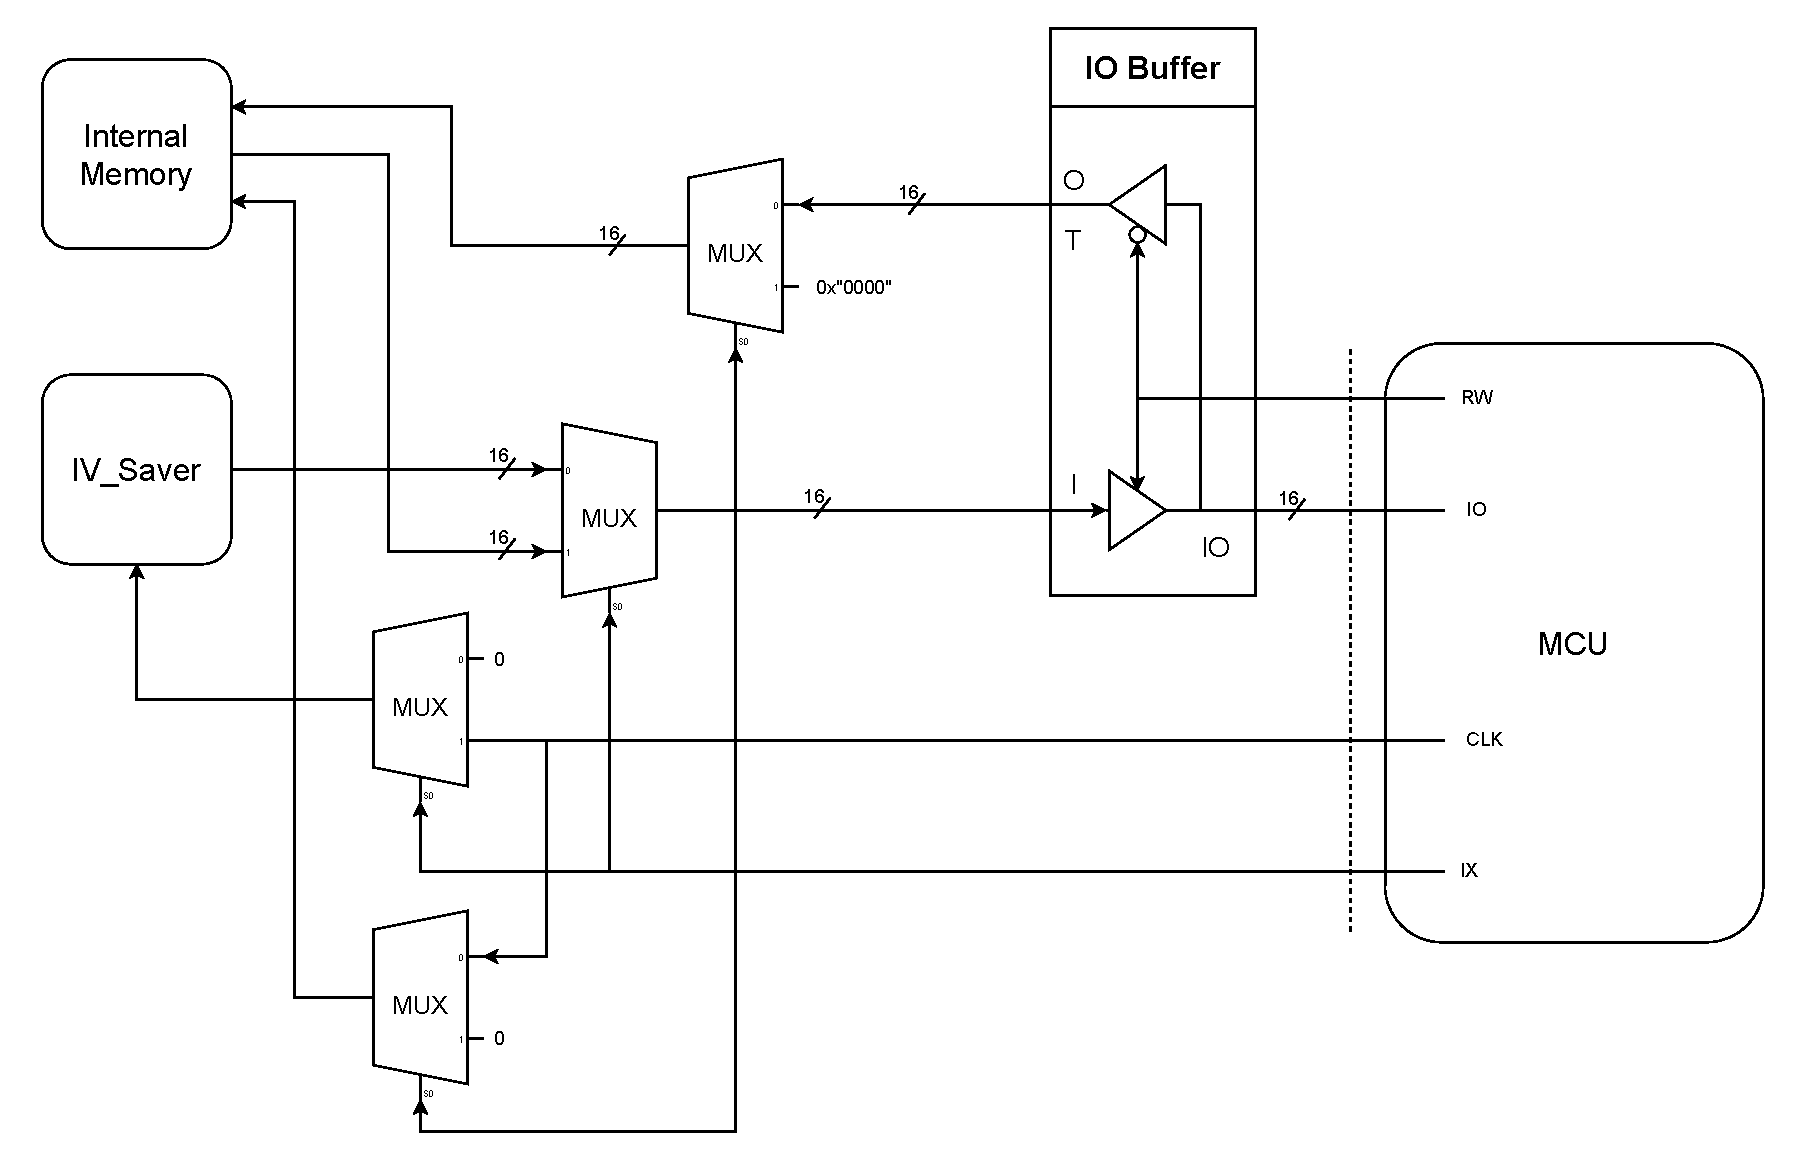
\includegraphics[clip, trim=0 0 0 0, width=1\textwidth]{Sections/7_SystemDesign/Figures/IXMUX_Functionality.pdf}
    \caption{A diagram showing how the IXMUX muxes the IO port dependant on the state of the IX pin, the MUXes set their output/input to 1 when IX is logical 1.}
    \label{fig_7_2_1.5_IXMUX_schematic}
\end{figure}

Functionally the IXMUX is made of 4 muxes, called XMEM\_CLK\_MUX, IMEM\_CLK\_MUX, o\_DATA\_IO\_MUX and o\_DATA\_IMEM\_MUX. These four muxes can be seen in listing \ref{lst:7_2_IXMUX}. INTERNAL is a constant that is '1' and EXTERNAL is a constant that is '0'.

\lstinputlisting[language=VHDL ,style = c,firstnumber=1, linerange=63-104, caption={VHDL code for the four MUXes that the IXMUX is made from.}, label={lst:7_2_IXMUX}]{Sections/7_SystemDesign/Code/IXMUX.vhd}

One thing to take notice of is that the CLK MUXes are synchronous. They will only change state on the rising edge of the \SIQ{200}{\mega\hertz} master clock. This is done to tell the syntheziser that these MUXes are time sensitive. This tells the software to place these elements close together on the chip. The data MUXes can also be made synchronous if desired, it has been tested both with and without and works well in both cases. 